%======================
%   P3M code
%======================
\subsection{$\mathrm{P^{3}M}$ code} \label{subsec:P3M}
In this section, we explain the usage of a FDPS extension ``Particle Mesh" (hereafter \textsf{PM}) using a sample program for $\mathrm{P^{3}M}$(Particle-Particle-Particle-Mesh) method. The sample code calculates the crystal energy of sodium chloride (NaCl) crystal using the $\mathrm{P^{3}M}$ method and compares the result with the analytical solution. In the $\mathrm{P^{3}M}$ method, the calculation of force and potential energy is performed by splitting into Particle-Particle(PP) part and Particle-Mesh(PM) part. In this sample code, the PP part is calculated by using FDPS standard features and the PM part is computed by using a FDPS extension ``PM". Note that the detail of the extension ``\textsf{PM}" is described in \S~9.2 of the specification of FDPS and please see it for detail.

\subsubsection{Location of sample code and working directory}
The sample code is placed at \dirNamePPPMSample.
Change the current directory to there.
\ifCpp
\begin{screen}
\begin{verbatim}
$ cd (FDPS)/sample/c++/p3m
\end{verbatim}
\end{screen}
The sample code consists of \texttt{main.cpp} and a Makefile for GCC, \texttt{Makefile}.
\endifCpp
\ifFtn
\begin{screen}
\begin{verbatim}
$ cd (FDPS)/sample/fortran/p3m
\end{verbatim}
\end{screen}
The sample code consists of \texttt{user\_defined.F90} where user-defined types and interaction functions are implemented, \texttt{f\_main.F90} where the other parts of the user code are implemented, and Makefiles for GCC and intel compiler, \texttt{Makefile} and \texttt{Makefile.intel}.
\endifFtn
\ifC
\begin{screen}
\begin{verbatim}
$ cd (FDPS)/sample/c/p3m
\end{verbatim}
\end{screen}
The sample code consists of \texttt{user\_defined.h} where user-defined types are implemented, \texttt{user\_defined.c} where interaction functions are implemented, \texttt{c\_main.c} where the other parts of the user code are implemented, and a Makefile for GCC, \texttt{Makefile}.
\endifC

%########################
%   User-defined types
%########################
\subsubsection{User-defined types}
In this section, we describe \structures that you need to define in order to perform $\mathrm{P^{3}M}$ calculation using FDPS.

%-----------------------
%   FullParticle type
%-----------------------
\subsubsubsection{FullParticle type}
You must define a \textsf{FullParticle} type. Listing~\ref{p3m_FP} shows the implementation of \textsf{FullParticle} type in the sample code. \textsf{FullParticle} type must have all physical quantities required to perform a calculation with $\mathrm{P^{3}M}$ method.
\ifCpp
It must have the following member functions:
\begin{description}[leftmargin=*,itemsep=-1ex,style=nextline]
\item[\texttt{getCharge()}] required for FDPS to get the charge of particles
\item[\texttt{getChargeParticleMesh()}] required for the \textsf{PM} module of FDPS to get the charge of particles
\item[\texttt{getPos()}] required for FDPS to get the position of particles
\item[\texttt{getRSearch()}] required for FDPS to get the cutoff radius
\item[\texttt{setPos()}] required for FDPS to write the positions of particles recorded in \textsf{FullParticle} object
\item[\texttt{copyFromForce()}] required for FDPS to copy data form \textsf{Force} object
\item[\texttt{copyFromForceParticleMesh()}] required for the \textsf{PM} module to write the result of Force calculation to \textsf{FullParticle} object
\end{description}
Note that \texttt{copyFromForce()} and \texttt{copyFromForceParticleMesh()} are empty functions in this sample code. This is because the sample code explicitly copy data from \textsf{Force} objects to \textsf{FullParticle} object using APIs such as \texttt{getForce()} (explained later). 
\endifCpp

\ifCpp
\lstinputlisting[linerange={90-118},caption=FullParticle type,label=p3m_FP]{../../../../sample/c++/p3m/main.cpp}
\endifCpp
\ifFtn
\lstinputlisting[linerange={18-30},caption=FullParticle type,label=p3m_FP]{../../../../sample/fortran/p3m/user_defined.F90}
\endifFtn
\ifC
\lstinputlisting[linerange={21-32},caption=FullParticle type,label=p3m_FP]{../../../../sample/c/p3m/user_defined.h}
\endifC

\ifIF
At first, users must specify which user-defined type this \structure corresponds to. The following directive specify that this \structure is a \textsf{FullParticle} type:
\endifIF
\ifFtn
\begin{screen}
\begin{verbatim}
type, public, bind(c) :: nbody_fp !$fdps FP
\end{verbatim}
\end{screen}
\endifFtn
\ifC
\begin{screen}
\begin{verbatim}
typedef struct fp_nbody { //$fdps FP
\end{verbatim}
\end{screen}
\endifC
\ifIF
In this $\mathrm{P^{3}M}$ code, the interaction force is long-range force with cutoff. Therefore, a cutoff radius is also necessary physical quantity in addition to the position and mass (charge). In the current version of FDPS, designation of cutoff radius is done by the same directive used for search radius (see \S~\ref{subsec:how_to_use_SPH_code}). We can tell FDPS which member variables represent these necessary quantities in the following way:
\endifIF
\ifFtn
\begin{screen}
\begin{verbatim}
real(kind=c_double) :: m !$fdps charge
real(kind=c_double) :: rc !$fdps rsearch
type(fdps_f64vec) :: x !$fdps position
\end{verbatim}
\end{screen}
\endifFtn
\ifC
\begin{screen}
\begin{verbatim}
double mass; //$fdps charge
double rcut; //$fdps rsearch     
fdps_f64vec pos; //$fdps position
\end{verbatim}
\end{screen}
\endifC
\ifIF
\textsf{FullParticle} type copies data from a \textsf{Force} type. Users must specify how the data is copied by using of directives. Also, when using the FDPS extension ``PM" to calculate interaction, users must specify how a \textsf{FullParticle} type receives the result of interaction calculation from a ``PM" module. In this sample code, there directives are written as follows.
\endifIF
\ifFtn
\begin{screen}
\begin{verbatim}
!$fdps copyFromForce nbody_pp_results (pot,pot) (agrv,agrv)
!$fdps copyFromForcePM agrv_pm
\end{verbatim}
\end{screen}
\endifFtn
\ifC
\begin{screen}
\begin{verbatim}
//$fdps copyFromForce force_pp (pot,pot) (acc,acc)  
//$fdps copyFromForcePM acc_pm                      
\end{verbatim}
\end{screen}
\endifC


%------------------------------
%   EssentialParticleI type
%------------------------------
\subsubsubsection{EssentialParticleI type}
You must define a \textsf{EssentialParticleI} type. \textsf{EssentialParticleI} type must have member variables that store all physical quantities necessary for an $i$ particle to perform the PP part of the Force calculation. In the sample code, it is also used as \textsf{EssentialParticleJ} type. Therefore, it should have member variables that store all physical quantities necessary for a $j$ particle to perform the PP part of the Force calculation. Listing~\ref{p3m_EP} shows the implementation of \textsf{EssentialParticleI} type in the sample code. 
\ifCpp
\textsf{EssentialParticleI} type needs to have member function \texttt{copyFromFP()} to copy data from \textsf{FullParticle} object described above. In addition, it must have \texttt{getCharge()} (returns the charges of particles), \texttt{getPos()} (returns the positions of particles), \texttt{getRSearch()} (returns the cutoff radius of particles), and \texttt{setPos()} (sets the positions of particles).
\endifCpp

\ifCpp
\lstinputlisting[linerange={121-147},caption=EssentialParticleI type,label=p3m_EP]{../../../../sample/c++/p3m/main.cpp}
\endifCpp
\ifFtn
\lstinputlisting[linerange={33-39},caption=EssentialParticleI型,label=p3m_EP]{../../../../sample/fortran/p3m/user_defined.F90}
\endifFtn
\ifC
\lstinputlisting[linerange={35-41},caption=EssentialParticleI型,label=p3m_EP]{../../../../sample/c/p3m/user_defined.h}
\endifC

\ifIF
At first, users must tell FDPS this \structure corresponds to \textsf{EssentialParticleI} and \textsf{EssentialParticleJ} types using a directive. This is done as follows.
\endifIF
\ifFtn
\begin{screen}
\begin{verbatim}
type, public, bind(c) :: nbody_ep !$fdps EPI,EPJ
\end{verbatim}
\end{screen}
\endifFtn
\ifC
\begin{screen}
\begin{verbatim}
typedef struct ep_nbody { //$fdps EPI,EPJ
\end{verbatim}
\end{screen}
\endifC
\ifIF
Next, users must specify which member variable corresponds to which necessary quantity using a directive. As described in the explanation of \textsf{FullParticle} type, cutoff radius is also necessary quantity. Therefore, the following directives are written in this sample code.
\endifIF
\ifFtn
\begin{screen}
\begin{verbatim}
real(kind=c_double) :: m !$fdps charge
real(kind=c_double) :: rc !$fdps rsearch
type(fdps_f64vec) :: x !$fdps position
\end{verbatim}
\end{screen}
\endifFtn
\ifC
\begin{screen}
\begin{verbatim}
double mass; //$fdps charge         
double rcut; //$fdps rsearch        
fdps_f64vec pos; //$fdps position   
\end{verbatim}
\end{screen}
\endifC
\ifIF
Both \textsf{EssentialParticleI} and \textsf{EssentialParticleJ} types copy data from a \textsf{FullParticle} type. Users must specify how data copy is performed by using of directives. In this sample code, the directives are written as follows.
\endifIF
\ifFtn
\begin{screen}
\begin{verbatim}
!$fdps copyFromFP nbody_fp (id,id) (m,m) (rc,rc) (x,x)
\end{verbatim}
\end{screen}
\endifFtn
\ifC
\begin{screen}
\begin{verbatim}
//$fdps copyFromFP fp_nbody (id,id) (mass,mass) (rcut,rcut) (pos,pos)
\end{verbatim}
\end{screen}
\endifC


%-----------------
%   Force type
%-----------------
\subsubsubsection{Force type}
You must define a \textsf{Force} type. \textsf{Force} type must have member variables that store the results of the PP part of the Force calculation. Listing~\ref{p3m_force} shows the implementation of \text{Force} type in this sample code. Because we consider Coulomb interaction only, one \textsf{Force} type is defined.
\ifCpp
\textsf{Force} type needs to have member function \texttt{clear()} to zero-clear or initialize member variables that store the results of accumulation operation.
\endifCpp

\ifCpp
\lstinputlisting[linerange={78-87},caption=Force type,label=p3m_force]{../../../../sample/c++/p3m/main.cpp}
\endifCpp
\ifFtn
\lstinputlisting[linerange={11-15},caption=Force型,label=p3m_force]{../../../../sample/fortran/p3m/user_defined.F90}
\endifFtn
\ifC
\lstinputlisting[linerange={14-18},caption=Force型,label=p3m_force]{../../../../sample/c/p3m/user_defined.h}
\endifC

\ifIF
At first, users must specify this \structure is a \textsf{Force} type using a directive. In this sample code, it is written as.
\endifIF
\ifFtn
\begin{screen}
\begin{verbatim}
type, public, bind(c) :: nbody_pp_results !$fdps Force
\end{verbatim}
\end{screen}
\endifFtn
\ifC
\begin{screen}
\begin{verbatim}
typedef struct force_pp { //$fdps Force
\end{verbatim}
\end{screen}
\endifC
\ifIF
Because this \structure is a \textsf{Force} type, users \ulBold{must} specify how member variables are initialized before interaction calculation via  directives. In this sample code, we adopt the default initialization for all of the member variables. This is realized by writing a FDPS directive with \texttt{clear} keyword only:
\endifIF
\ifFtn
\begin{screen}
\begin{verbatim}
!$fdps clear
\end{verbatim}
\end{screen}
\endifFtn
\ifC
\begin{screen}
\begin{verbatim}
//$fdps clear
\end{verbatim}
\end{screen}
\endifC


%---------------------
%   calcForceEpEp
%---------------------
\subsubsubsection{calcForceEpEp} \label{subsubsubsec:p3m_calcForceEpEp}
You must define an interaction function \textsf{calcForceEpEp}. \textsf{calcForceEpEp} must contain actual code for the PP part of the Force calculation and must be implemented as \procedure \describeForCpp{or functor (function object)}. Its arguments is an array of \textsf{EssentialParticleI} objects, the number of \textsf{EssentialParticleI} objects, an array of \textsf{EssentialParticleJ} objects, the number of \textsf{EssentialParticleJ} objects, and an array of \textsf{Force} objects. Listing~\ref{p3m_calcForceEpEp} shows the implementation of \textsf{calcForceEpEp} in this sample code. \describeForCpp{In the code, it is implemented as a functor.} 

\ifCpp
\lstinputlisting[linerange={150-174},caption=Interaction function calcForceEpEp,label=p3m_calcForceEpEp]{../../../../sample/c++/p3m/main.cpp}
\endifCpp
\ifFtn
\lstinputlisting[linerange={121-152},caption=Interaction function calcForceEpEp,label=p3m_calcForceEpEp]{../../../../sample/fortran/p3m/user_defined.F90}
\endifFtn
\ifC
\lstinputlisting[linerange={58-85},caption=Interaction function calcForceEpEp,label=p3m_calcForceEpEp]{../../../../sample/c/p3m/user_defined.c}
\endifC


% Cutoff functions
The PP part in the $\mathrm{P^{3}M}$ method is a two-body interaction with cutoff (i.e. the interaction is truncated if the distance between the particles is larger than the cutoff distance). Hence, cutoff functions (\texttt{S2\_pcut()}, \texttt{S2\_fcut()}) appears in the calculations of potential and acceleration. These cutoff functions must be the ones that are constructed assuming that the particle shape function is $S2(r)$, which is introduced by Hockney \& Eastwood (1988)(Eq.(8.3)) and takes the form of 
\begin{equation}
S2(r) = \left\{
\begin{array}{ll}
\dfrac{48}{\pi a^{4}}\left(\dfrac{a}{2}-r\right) & r < a/2, \\
0 & \mathrm{otherwise}.
\end{array}
\right.
\end{equation}
where $r$ is the distance from the center of a particle, $a$ is the scale length of the shape function. When assuming this shape function, the charge density distribution due to a particle, $\rho(r)$, is expressed as $\rho(r)=q\,S2(r)$, where $q$ is the charge of the particle. Thus, $S2(r)$ shape function gives linear density distribution. The reason why we have to use the cutoff functions that correspond to $S2(r)$ shape function is that the cutoff functions used in the PM part also assumes the $S2(r)$ shape function (the cutoff functions in the PM and PP parts should be consistent with each other).

% Implementation of cutoff functions
The cutoff functions must be defined by a user. Possible implementations for \texttt{S2\_pcut()} and \texttt{S2\_fcut()} are given at the beginning of the sample code (see the lines 22-72 in \texttt{main.cpp}). In these examples, we used Eqs.(8-72) and (8-75) in Hockney \& Eastwood (1988) and we define them such that the PP interaction takes of the form:
\begin{eqnarray}
\Phi_{\mathrm{PP}}(\bm{r}) & = & \dfrac{m}{|\bm{r}-\bm{r}'|}\mathtt{S2\_pcut}(\xi) \\
\bm{f}_{\mathrm{PP}}(\bm{r}) & = & \dfrac{m(\bm{r}-\bm{r}')}{|\bm{r}-\bm{r}'|^{3}}\mathtt{S2\_fcut}(\xi)
\end{eqnarray}
where $\xi = 2|\bm{r}-\bm{r}'|/a$.
In this sample code, $a$ is expressed as a variable \describeForEach{\texttt{rc}}{\texttt{rc}}{\texttt{rcut}}.

% About Self-interaction term
As is clear from Eq.(8-75) in Hockney \& Eastwood (1988), the mesh potential $\phi^{m}$ has a finite value at $r=0$ (we omit a factor $1/4\pi\varepsilon_{0}$ here):
\begin{equation}
\phi^{m}(0) = \dfrac{208}{70a}
\end{equation}
This term is taken into account the last line in the $i$-particle loop:
\ifCpp
\begin{lstlisting}
result[i].pot -= ep_i[i].m * (208.0/(70.0*ep_i[i].rc));
\end{lstlisting}
\endifCpp
\ifFtn
\begin{lstlisting}
f(i)%pot = f(i)%pot - ep_i(i)%m * (208.0d0/(70.0d0*ep_i(i)%rc))
\end{lstlisting}
\endifFtn
\ifC
\begin{lstlisting}
f[i].pot -= ep_i[i].mass * (208.0/(70.0*ep_i[i].rcut));
\end{lstlisting}
\endifC
Note that this term is necessary to match the numerical result with the analytical solution.

%---------------------
%   calcForceEpSp
%---------------------
\subsubsubsection{calcForceEpSp} \label{subsubsubsec:p3m_calcForceEpSp}
You must define an interaction function \textsf{calcForceEpSp}\footnote{As describe at the beginning of this section, the sample code uses $\mathrm{P^{3}M}$ for the calculation of interaction. In order to realize it using FDPS, we perform the calculation of interaction with the opening angle criterion $\theta$ of 0. Hence, particle-superparticle interaction should not occur. However, API \describeForEach{\texttt{calcForceAllAndWriteBack}}{\texttt{calc\_force\_all\_and\_write\_back}}{\texttt{fdps\_calc\_force\_all\_and\_write\_back}} requires a function pointer of a \procedure that calculates particle-superparticle interaction. Therefore, we defined \textsf{calcForceEpSp} here.}. \textsf{calcForceEpSp} must contain actual code for particle-superparticle interaction and must be implemented as \procedure \describeForCpp{or functor (function object)}. Its arguments is an array of \textsf{EssentialParticleI} objects, the number of \textsf{EssentialParticleI} objects, an array of \textsf{SuperParticleJ} objects, the number of \textsf{SuperParticleJ} objects, and an array of \textsf{Force} objects. Listing \ref{p3m_calcForceEpSp} shows the implementation of \textsf{calcForceEpSp} in the sample code.

\ifCpp
\lstinputlisting[linerange={175-195},caption=Interaction function calcForceEpSp,label=p3m_calcForceEpSp]{../../../../sample/c++/p3m/main.cpp}
\endifCpp
\ifFtn
\lstinputlisting[linerange={155-183},caption=Interaction function calcForceEpSp,label=p3m_calcForceEpSp]{../../../../sample/fortran/p3m/user_defined.F90}
\endifFtn
\ifC
\lstinputlisting[linerange={87-111},caption=Interaction function calcForceEpSp,label=p3m_calcForceEpSp]{../../../../sample/c/p3m/user_defined.c}
\endifC


%-----------------------------------
%   Main body of the sample code
%-----------------------------------
\subsubsection{Main body of the sample code}
In this section, we explain the main body of the sample code. Before going into details, we first give a simple explanation about the content and the structure of the sample code. As described in \S~\ref{subsec:P3M}, this code computes the crystal energy of NaCl crystal using the $\mathrm{P^{3}M}$ method and compares the result with the analytical solution. The NaCl crystal is expressed as an uniform grid of particles in this sample code. Na and Cl are placed in the staggered layout. Particles corresponding to Na has a positive charge, while those corresponding to Cl has a negative charge. We place a crystal expressed as an grid of charged particles into a periodic computational box of the sizes $[0,1)^{3}$ and calculates the crystal energy. The computational accuracy of the crystal energy should depend on the number of particles and the configuration of particles (to the grid used in the PM calculation). Hence, in the sample code, we measure the relative energy errors for a different set of these parameters and output the result of the comparisons into a file.

The structure of the sample code is as follows:
\begin{enumerate}[leftmargin=*,itemsep=-1ex,label={(\arabic*)}]
\item Create and initialize FDPS objects
\item Create a NaCl crystal for given number of particles and configuration (in \procedure \describeForEach{\texttt{NaCl\_IC()}}{\texttt{setup\_NaCl\_crystal()}}{\texttt{setup\_NaCl\_crystal()}})
\item Compute the potential energy of each particle by the $\mathrm{P^{3}M}$ method (\describeForEach{in \procedure \texttt{Nbody\_objs.calc\_gravity()}}{In \mainFuncName}{In \mainFuncName})
\item Compute the total energy of the crystal and compare it with the analytical solution (\procedure \texttt{calc\_energy\_error()})
\item Repeat (2)-(4)
\end{enumerate}

In the following, we explain in detail each steps described above.

\ifCpp
\subsubsection{Include header files}
In order to use the FDPS extension ``\textsf{PM}", we must include the header files \texttt{particle\_mesh.hpp} and \texttt{param\_fdps.h} as well as \texttt{particle\_simulator.hpp} (the last one is needed to use FDPS standard features). In addition, \texttt{param.h} is included because the sample code accesses a non-public constant \texttt{CUTOFF\_RADIUS}.
\begin{lstlisting}[caption=Include FDPS's header files]
#include <particle_simulator.hpp>
#include <particle_mesh.hpp>
#include <param.h>
#include <param_fdps.h>
\end{lstlisting}
\endifCpp
\ifFtn
\subsubsubsection{Creation of an object of type \texttt{fdps\_controller}}
In the FDPS Fortran interface, all APIs of FDPS are provided as member functions in the class \texttt{FDPS\_controller}. This class is defined in the module \texttt{fdps\_module} in \texttt{FDPS\_module.F90}. Thus, in order to use APIs, the user must create an object of type \texttt{FDPS\_controller}. In this sample, the object of type \texttt{FDPS\_controller},  \texttt{fdps\_ctrl}, is created in the main routine. Thus, in the following examples, APIs of FDPS are called as a member function of this object.

\begin{lstlisting}[caption=Creation of an object of type \texttt{fdps\_controller}]
subroutine f_main()
   use fdps_module
   implicit none
   !* Local variables
   type(fdps_controller) :: fdps_ctrl
    
   ! Do something
   
end subroutine f_main    
\end{lstlisting}

Note that the code shown above is an only necessary part from the sample code. 
\endifFtn
\ifC
\subsubsubsection{Including the header file of FDPS C interface}
To make the standard features of FDPS available, we must include header file  \texttt{FDPS\_c\_if.h}.
\begin{lstlisting}[caption=Including header file \texttt{FDPS\_c\_if.h}]
#include "FDPS_c_if.h"
\end{lstlisting}
\endifC


\subsubsubsection{Initialization and Termination of FDPS}
First, you must initialize FDPS by the following code.
\ifCpp
\begin{lstlisting}[caption=Initialization of FDPS]
PS::Initialize(argc, argv);
\end{lstlisting}
\endifCpp
\ifFtn
\begin{lstlisting}[caption=Initialization of FDPS]
fdps_ctrl%ps_initialize();
\end{lstlisting}
\endifFtn
\ifC
\begin{lstlisting}[caption=Initialization of FDPS]
fdps_initialize();
\end{lstlisting}
\endifC


Once started, FDPS should be terminated explicitly. In this sample, FDPS is terminated just before the termination of the program. Hence, you need to write the following code at the end of the main function.
\ifCpp
\begin{lstlisting}[caption=Termination of FDPS]
PS::Finalize();
\end{lstlisting}
\endifCpp
\ifFtn
\begin{lstlisting}[caption=Termination of FDPS]
fdps_ctrl%ps_finalize();
\end{lstlisting}
\endifFtn
\ifC
\begin{lstlisting}[caption=Termination of FDPS]
fdps_finalize();
\end{lstlisting}
\endifC


\subsubsubsection{Creation and initialization of FDPS objects}
After the initialization of FDPS, a user need to create the objects used to talk to FDPS. In this section, we describe how to create and initialize these objects.

\subsubsubsubsection{Creation of necessary FDPS objects}
\ifCpp
In the calculation using the $\mathrm{P^{3}M}$ method, we must create objects of the \textsf{ParticleSystem} class and the \textsf{DomainInfo} class. In addition, objects of the \textsf{TreeForForceLong} class and the \textsf{ParticleMesh} class are need to calculate the PP and PM parts of the force calculation. In this sample code, these objects are grouped into \texttt{Nbody\_Objects} class. The following code is the implementation of the \texttt{Nbody\_Objects} class.
\begin{lstlisting}[caption=\texttt{Nbody\_Objects} class]
class Nbody_Objects {
   public:
      PS::ParticleSystem<Nbody_FP> system;
      PS::DomainInfo dinfo;
      PS::TreeForForceLong<Nbody_PP_Results, Nbody_EP, Nbody_EP>::MonopoleWithCutoff pp_tree;
      PS::PM::ParticleMesh pm;
}
\end{lstlisting}
In this sample, a object of the \texttt{Nbody\_Objects} class is created as a local variable in the main function:
\begin{lstlisting}[caption=Creation of a \texttt{Nbody\_Objects}-class object]
Nbody_Objects Nbody_objs;
\end{lstlisting}
\endifCpp

\ifIF
In the calculation using the $\mathrm{P^{3}M}$ method, we must create \textsf{ParticleSystem} and \textsf{DomainInfo} objects. In addition, \textsf{Tree} and \textsf{ParticleMesh} objects are also needed to calculate the PP and PM parts of the force calculation.
\endifIF
\ifFtn
\begin{lstlisting}[caption=Creation of FDPS objects]
call fdps_ctrl%create_psys(psys_num,'nbody_fp')
call fdps_ctrl%create_dinfo(dinfo_num)
call fdps_ctrl%create_pm(pm_num)
call fdps_ctrl%create_tree(tree_num, &                                                  
                           "Long,nbody_pp_results,nbody_ep,nbody_ep,MonopoleWithCutoff")
\end{lstlisting}
Note that the code snippet shown above differs from the actual sample code.
\endifFtn
\ifC
\begin{lstlisting}[caption=Creation of FDPS objects]
fdps_create_psys(&psys_num,"fp_nbody");
fdps_create_dinfo(&dinfo_num);
fdps_create_pm(&pm_num);
fdps_create_tree(&tree_num,
                 "Long,force_pp,ep_nbody,ep_nbody,MonopoleWithCutoff");
\end{lstlisting}
Note that the code snippet shown above differs from the actual sample code.
\endifC


\subsubsubsubsection{Initialization of FDPS objects}
After the creation of FDPS objects, you must initialize these objects before you use them in a user code. In the following, we explain how to initialize each object.

\begin{description}[leftmargin=*,font=\normalfont\slshape]
\item[(i) Initialization of a \textsf{ParticleSystem} object]
A \textsf{ParticleSystem} object is initialized as follows:
\ifCpp
\begin{lstlisting}[caption=Initialization of a \textsf{ParticleSystem} object]
Nbody_objs.system.initialize();
\end{lstlisting}
\endifCpp
\ifFtn
\begin{lstlisting}[caption=Initialization of a \textsf{ParticleSystem} object]
call fdps_ctrl%init_psys(psys_num)
\end{lstlisting}
\endifFtn
\ifC
\begin{lstlisting}[caption=Initialization of a \textsf{ParticleSystem} object]
fdps_init_psys(psys_num);
\end{lstlisting}
\endifC
This is done in the \mainFunc in the sample code.

\item[(ii) Initialization of a \textsf{DomainInfo} object]
A \textsf{DomainInfo} object is initialized as follows:
\ifCpp
\begin{lstlisting}[caption=Initialization of a \textsf{DomainInfo} object]
Nbody_objs.dinfo.initialize();
\end{lstlisting}
\endifCpp
\ifFtn
\begin{lstlisting}[caption=Initialization of a \textsf{DomainInfo} object]
call fdps_ctrl%init_dinfo(dinfo_num,coef_ema)
\end{lstlisting}
\endifFtn
\ifC
\begin{lstlisting}[caption=Initialization of a \textsf{DomainInfo} object]
fdps_init_dinfo(dinfo_num,coef_ema);
\end{lstlisting}
\endifC
This is done in the \mainFunc in the sample code.

After the initialization, you need to specify the boundary condition and the size of the simulation box through APIs \describeForEach{\texttt{setBoundaryCondition}}{\texttt{set\_boundary\_condition}}{\texttt{fdps\_set\_boundary\_condition}} and \describeForEach{\texttt{setPosRootDomain}}{\texttt{set\_pos\_root\_domain}}{\texttt{fdps\_set\_pos\_root\_domain}}. In the sample code, these procedures are performed in \procedure \describeForEach{\texttt{NaCl\_IC()}}{\texttt{setup\_NaCl\_crystal}}{\texttt{setup\_NaCl\_crystal}} that sets up the distribution of particles:
\ifCpp
\begin{lstlisting}
dinfo.setBoundaryCondition(PS::BOUNDARY_CONDITION_PERIODIC_XYZ);
dinfo.setPosRootDomain(PS::F64vec(0.0,0.0,0.0),
                       PS::F64vec(1.0,1.0,1.0));
\end{lstlisting}
\endifCpp
\ifFtn
\begin{lstlisting}
call fdps_ctrl%set_boundary_condition(dinfo_num,fdps_bc_periodic_xyz)
pos_ll%x = 0.0d0; pos_ll%y = 0.0d0; pos_ll%z = 0.0d0
pos_ul%x = 1.0d0; pos_ul%y = 1.0d0; pos_ul%z = 1.0d0
call fdps_ctrl%set_pos_root_domain(dinfo_num,pos_ll,pos_ul)
\end{lstlisting}
\endifFtn
\ifC
\begin{lstlisting}
fdps_set_boundary_condition(dinfo_num,FDPS_BC_PERIODIC_XYZ);
fdps_f32vec pos_ll, pos_ul;
pos_ll.x = 0.0; pos_ll.y = 0.0; pos_ll.z = 0.0;
pos_ul.x = 1.0; pos_ul.y = 1.0; pos_ul.z = 1.0;
fdps_set_pos_root_domain(dinfo_num,&pos_ll,&pos_ul);
\end{lstlisting}
\endifC


\item[(iii) Initialization of a \describeForEach{\textsf{TreeForForceLong}}{\textsf{Tree}}{\textsf{Tree}} object]
A \describeForEach{\textsf{TreeForForceLong}}{\textsf{Tree}}{\textsf{Tree}} object is initialized by API \describeForEach{\texttt{initialize}}{\texttt{init\_tree}}{\texttt{fdps\_init\_tree}}:
\ifCpp
\begin{lstlisting}[caption=Initialization of a \textsf{TreeForForceLong} object]
void init_tree() {
   PS::S32 numPtclLobal = system.getNumberOfParticleLobal();
   PS::U64 ntot = 3 * numPtclLobal;
   pp_tree.initialize(ntot,0.0);
}; 
\end{lstlisting}
\endifCpp
\ifFtn
\begin{lstlisting}[caption=Initialization of a \textsf{Tree} object]
call fdps_ctrl%init_tree(tree_num,3*nptcl_loc,theta, &
                         n_leaf_limit,n_group_limit)
\end{lstlisting}
\endifFtn
\ifC
\begin{lstlisting}[caption=Initialization of a \textsf{Tree} object]
fdps_init_tree(tree_num,3*nptcl_loc,theta,
               n_leaf_limit,n_group_limit);
\end{lstlisting}
\endifC

You need to give a rough number of particles to this API as the \describeForEach{first}{second}{second} argument. Here, we set three times the number of local particles at the time of calling. The \describeForEach{second}{third}{third} argument of this API \describeForEach{is an optional argument and}{is an optional argument and}{} represents the opening angle criterion $\theta$ for the tree method. In the sample, we do not use the tree method in the PP part of the force calculation. Therefore, we set $\theta=0$.

\ifCpp
In this sample code, a \textsf{TreeForForceLong} object is initialized within the function \texttt{Nbody\_objs.init\_tree()} (see the main function).
\begin{lstlisting}
if (is_tree_initialized == false) {
   Nbody_objs.init_tree();
   is_tree_initialized = true;
}
\end{lstlisting}
where the \texttt{if} statement above is necessary because the initialization should be done only once in the program (otherwise, the program will fail).
\endifCpp

\item[(iv) Initialization of a \textsf{ParticleMesh} object] No explicit initialization is needed.

\end{description}

\subsubsubsection{Generation of a distribution of particles}
In this section, we explain \procedure \describeForEach{\texttt{NaCl\_IC}}{\texttt{setup\_NaCl\_crystal}}{\texttt{setup\_NaCl\_crystal}} that generates a distribution of particles, and FDPS APIs called within it. Given the number of particles per one space dimension and the position of the particle that is nearest to the origin $(0,0,0)$, \procedure \describeForEach{\texttt{NaCl\_IC}}{\texttt{setup\_NaCl\_crystal}}{\texttt{setup\_NaCl\_crystal}} makes a three-dimensional uniform grid of particles. These parameters are specified through an object of \structure \describeForEach{\texttt{Crystal\_Parameters}}{\texttt{crystal\_parameters}}{\texttt{crystal\_parameters}}, \texttt{NaCl\_params}:
\ifCpp
\begin{lstlisting}
class Crystal_Parameters
{
   public:
      PS::S32 numPtcl_per_side;
      PS::F64vec pos_vertex;
};
/* In main function */
Crystal_Parameters NaCl_params;
NaCl_IC(Nbody_objs.system,
        Nbody_objs.dinfo,
        NaCl_params);
\end{lstlisting}
\endifCpp
\ifFtn
\begin{lstlisting}
! In user_defined.F90
type, public, bind(c) :: crystal_parameters
   integer(kind=c_int) :: nptcl_per_side
   type(fdps_f64vec) :: pos_vertex
end type crystal_parameters
! In f_main.F90
type(crystal_parameters) :: NaCl_params
call setup_NaCl_crystal(fdps_ctrl, &
                        psys_num,  &
                        dinfo_num, &
                        NaCl_params)
\end{lstlisting}
\endifFtn
\ifC
\begin{lstlisting}
// In user_defined.h
typedef struct crystal_parameters {
   int nptcl_per_side;
   fdps_f64vec pos_vertex;
} Crystal_parameters;
// In c_main.c
Crystal_parameters NaCl_params;
setup_NaCl_crystal(psys_num, dinfo_num, NaCl_params);
\end{lstlisting}
\endifC


In the first half of \procedure \describeForEach{\texttt{NaCl\_IC}}{\texttt{setup\_NaCl\_crystal}}{\texttt{setup\_NaCl\_crystal}}, it makes an uniform grid of particles based on the value of \texttt{NaCl\_params}. In this process, we scale the particle charge $m$ to satisfy the relation
\begin{equation}
\dfrac{2Nm^{2}}{R_{0}}=1,
\end{equation}
where $N$ is the total number of molecules (the total number of atomic particles is $2N$) and $R_{0}$ is the distance to the nearest particle. This scaling is introduced just for convenience: The crystal energy can be written analytically as
\begin{equation}
E = - \dfrac{N\alpha m^{2}}{R_{0}},
\end{equation}
where $\alpha$ is the Madelung constant and $\alpha\approx 1.747565$ for the NaCl crystal (e.g. see \href{http://as.wiley.com/WileyCDA/WileyTitle/productCd-EHEP000803.html}{Kittel (2004) "Introduction to Solid State Physics"}). Thus, the crystal energy depends on the total number of particles. This is inconvenient when comparing the calculation result with the analytical solution. By scaling the particle charge as described above, the crystal energy becomes independent from $N$.

After generating a particle distribution, this function performs domain decomposition and particle exchange using FDPS APIs. In the following, we explain these APIs.

\subsubsubsubsection{Domain Decomposition}
API \describeForEach{\texttt{decomposeDomainAll}}{\texttt{decompose\_domain\_all}}{\texttt{fdps\_decompose\_domain\_all}} of the \textsf{DomainInfo} object is used to perform domain decomposition based on the current distribution of particles:
\ifCpp
\begin{lstlisting}[caption=Domain Decomposition]
dinfo.decomposeDomainAll(system);
\end{lstlisting}
Note that this API needs a \textsf{ParticleSystem} object as the argument to get the information of particle distribution.
\endifCpp
\ifFtn
\begin{lstlisting}[caption=Domain Decomposition]
call fdps_ctrl%decompose_domain_all(dinfo_num,psys_num)
\end{lstlisting}
\endifFtn
\ifC
\begin{lstlisting}[caption=Domain Decomposition]
fdps_decompose_domain_all(dinfo_num,psys_num);
\end{lstlisting}
\endifC


\subsubsubsubsection{Particle Exchange}
API \describeForEach{\texttt{exchangeParticle}}{\texttt{exchange\_particle}}{\texttt{fdps\_exchange\_particle}} of the \textsf{ParticleSystem} object is used to exchange particles based on the current decomposed domains:
\ifCpp
\begin{lstlisting}[caption=Particle Exchange]
system.exchangeParticle(dinfo);
\end{lstlisting}
Note that this API needs a \textsf{DomainInfo} object as the argument to get the domain information.
\endifCpp
\ifFtn
\begin{lstlisting}[caption=Particle Exchange]
call fdps_ctrl%exchange_particle(psys_num,dinfo_num)
\end{lstlisting}
\endifFtn
\ifC
\begin{lstlisting}[caption=Particle Exchange]
fdps_exchange_particle(psys_num,dinfo_num);
\end{lstlisting}
\endifC



\subsubsubsection{Interaction Calculation}
After these procedures are completed, we must perform the interaction calculation.
\ifCpp
In the sample code, it is performed in the main function by calling the function \texttt{Nbody\_objs.calc\_gravity()}:
\begin{lstlisting}[caption=Execution of interaction calculation]
Nbody_objs.calc_gravity();
\end{lstlisting}

The function \texttt{Nbody\_objs.calc\_gravity()} consists of (i) zero-clear of potential energy and acceleration of each particle, (ii) calculation of the PM part, and (iii) calculation of the PP part:
\begin{lstlisting}[caption=Interaction calculation]
void calc_gravity() {
   //* Local variables
   PS::S32 numPtclLocal = system.getNumberOfParticleLocal();

   //* Reset potential and accelerations
   for (PS::S32 i=0; i<numPtclLocal; i++) {
      system[i].pot  = 0.0;
      system[i].agrv = 0.0;
   }

   //=================
   //* [1] PM part 
   //=================
   pm.setDomainInfoParticleMesh(dinfo);
   pm.setParticleParticleMesh(system);
   pm.calcMeshForceOnly();
   for (PS::S32 i=0; i<numPtclLocal; i++) {
      PS::F32vec x32 = system[i].x;
      system[i].pot  -= pm.getPotential(x32);
      system[i].agrv -= pm.getForce(x32);
   }

   //=================
   //* [2] PP part 
   //=================
   pp_tree.calcForceAll(Calc_force_ep_ep(),
                        Calc_force_ep_sp(),
                        system, dinfo);
   for (PS::S32 i=0; i<numPtclLocal; i++) {
      Nbody_PP_Results result = pp_tree.getForce(i);
      system[i].pot  += result.pot;
      system[i].agrv += result.agrv;
   }
};
\end{lstlisting}

The code shown below is the PM part of the Force calculation (hereafter PM calculation). In order to perform the PM calculation, the \textsf{ParticleMesh} object \texttt{pm} must have information about the domain and the particles in advance. Therefore, \texttt{setDomainInfoParticleMesh} and \texttt{setParticleParticleMesh} methods are first called to give these information to the object \texttt{pm}. Now, the object \texttt{pm} are ready to perform the PM calculation. In the sample code, the PM calculation is performed by \texttt{calcMeshForceOnly} method. Then, \texttt{getPotential} and \texttt{getForce} methods are called to obtain the potential and acceleration at the particle position. They are stored to the \textsf{FullParticle} type object \texttt{system}. \textit{\textbf{Note that the accumulation operation is done by the operator \texttt{-=}}}. The reason why we use \texttt{-=} instead of \texttt{+=} is that the FDPS extension ``\textsf{PM}" computes the potential energy assuming gravity. In other words, the FDPS extension ``\textsf{PM}" treats a charge with $m(>0)$ creates negative potential. Hence, \textit{\textbf{we need to invert the signs of potential energy and acceleration}} in order to use the FDPS extension ``\textsf{PM}" for the Coulomb interaction calculation.
\begin{lstlisting}[caption=PM part of Force calculation]
pm.setDomainInfoParticleMesh(dinfo);
pm.setParticleParticleMesh(system);
pm.calcMeshForceOnly();
for (PS::S32 i=0; i<numPtclLocal; i++) {
   PS::F32vec x32 = system[i].x;
   system[i].pot  -= pm.getPotential(x32);
   system[i].agrv -= pm.getForce(x32);
}
\end{lstlisting}

Next, we shows the PP part of the Force calculation in the following. The \texttt{calcForceAll} method of the \textsf{TreeForForceLong} class is used to calculation the PP part (we do not use the \texttt{calcForceAllAndWriteBack} method because this method zero-clears the results of the PM calculation stored the \textsf{FullParticle} object). Then, the \texttt{getForce} method is used to obtain the potential energy and the acceleration at the particle position and they are accumulated to the \textsf{FullParticle}-type object \texttt{system}.
\begin{lstlisting}[caption=PP part of Force calculation]
pp_tree.calcForceAll(Calc_force_ep_ep(),
                     Calc_force_ep_sp(),
                     system, dinfo);
for (PS::S32 i=0; i<numPtclLocal; i++) {
   Nbody_PP_Results result = pp_tree.getForce(i);
   system[i].pot  += result.pot;
    system[i].agrv += result.agrv;
}
\end{lstlisting}
\endifCpp

\ifIF
In the sample code, it is performed in the \mainFunc.
\endifIF
\ifFtn
\begin{lstlisting}[caption=Interaction calculation]
!* [4] Compute force and potential with P^{3}M method
!* [4-1] Get the pointer to FP and # of local particles
nptcl_loc = fdps_ctrl%get_nptcl_loc(psys_num)
call fdps_ctrl%get_psys_fptr(psys_num,ptcl)
!* [4-2] PP part
pfunc_ep_ep = c_funloc(calc_force_ep_ep)
pfunc_ep_sp = c_funloc(calc_force_ep_sp)
call fdps_ctrl%calc_force_all_and_write_back(tree_num,    &
                                             pfunc_ep_ep, &
                                             pfunc_ep_sp, &
                                             psys_num,    &
                                             dinfo_num)
!* [4-3] PM part
call fdps_ctrl%calc_pm_force_all_and_write_back(pm_num,   &
                                                psys_num, &
                                                dinfo_num)
do i=1,nptcl_loc
   pos32 = ptcl(i)%x
   call fdps_ctrl%get_pm_potential(pm_num,pos32,ptcl(i)%pot_pm)
end do
!* [4-4] Compute the total acceleration and potential
do i=1,nptcl_loc
   ptcl(i)%pot  = ptcl(i)%pot  - ptcl(i)%pot_pm
   ptcl(i)%agrv = ptcl(i)%agrv - ptcl(i)%agrv_pm
end do
\end{lstlisting}
\endifFtn
\ifC
\begin{lstlisting}[caption=Interaction calculation]
// [4] Compute force and potential with P^{3}M method
// [4-1] Get the pointer to FP and # of local particles
int nptcl_loc = fdps_get_nptcl_loc(psys_num);
FP_nbody *ptcl = (FP_nbody *) fdps_get_psys_cptr(psys_num);
// [4-2] PP part
fdps_calc_force_all_and_write_back(tree_num,
                                   calc_force_ep_ep,
                                   calc_force_ep_sp,
                                   psys_num,
                                   dinfo_num,
                                   true,
                                   MAKE_LIST);
// [4-3] PM part
fdps_calc_pm_force_all_and_write_back(pm_num,
                                      psys_num,
                                      dinfo_num);
int i;
for (i = 0; i < nptcl_loc; i++) {
   fdps_f32vec pos32;
   pos32.x = ptcl[i].pos.x;
   pos32.y = ptcl[i].pos.y;
   pos32.z = ptcl[i].pos.z;
   fdps_get_pm_potential(pm_num,&pos32,&ptcl[i].pot_pm);
}
// [4-4] Compute the total acceleration and potential
for (i = 0; i < nptcl_loc; i++) {
   ptcl[i].pot -= ptcl[i].pot_pm;
   ptcl[i].acc.x -= ptcl[i].acc_pm.x;
   ptcl[i].acc.y -= ptcl[i].acc_pm.y;
   ptcl[i].acc.z -= ptcl[i].acc_pm.z;
}
\end{lstlisting}
\endifC
\ifIF
We use API \describeForEach{}{\texttt{calc\_force\_all\_and\_write\_back}}{\texttt{fdps\_calc\_force\_all\_and\_write\_back}} for the PP part and API \describeForEach{}{\texttt{calc\_pm\_force\_all\_and\_write\_back}}{\texttt{fdps\_calc\_pm\_force\_all\_and\_write\_back}} for the PM part. After calculating the PM part, the total acceleration and total potential are computed. Please note that this summation is done by \uwave{{\textbf{subtraction}}}. The reason why we use subtraction is that the FDPS extension ``\textsf{PM}" computes the potential energy assuming gravity. In other words, the FDPS extension ``\textsf{PM}" treats a charge with $m(>0)$ creates negative potential. Hence, \textit{\textbf{we need to invert the signs of potential energy and acceleration}} in order to use the FDPS extension ``\textsf{PM}" for the Coulomb interaction calculation.

\endifIF


\subsubsubsection{Calculation of relative energy error}
The relative error of the crystal energy is computed in the function \texttt{calc\_energy\_error()}, where we assume that the analytical solution is $E_{0}\equiv 2E =-1.7475645946332$, which is numerically evaluated by the $\mathrm{PM^{3}}$(Particle-Mesh Multipole Method).

\subsubsection{Compile}
Before compiling your program, you need to install the \href{http://www.fftw.org}{FFTW(Fast Fourier Transform in the West) library}. Then, edit the file \texttt{Makefile} in the working directory to set the PATHs of the locations of FFTW and FDPS to the variables \texttt{FFTW\_LOC} and \texttt{FDPS\_LOC}. After that, run \texttt{make}.
\begin{screen}
\begin{verbatim}
$ make
\end{verbatim}
\end{screen}
The execution file \texttt{p3m.x} will be created in the directory \texttt{work} if the compilation is succeeded.

\subsubsection{Run}
You must run your program using MPI with the number of MPI processes is equal to or greater than 2, because of the specification of FDPS extensions. Therefore, you should run the following command:
\begin{screen}
\begin{verbatim}
$ MPIRUN -np NPROC ./p3m.x
\end{verbatim}
\end{screen}
where ``MPIRUN" represents the command to run your program using MPI such as \texttt{mpirun} or \texttt{mpiexec}, and ``NPROC" is the number of MPI processes.

\subsubsection{Check the result}
After the program ended, a file that records the relative error of the crystal energy is output in the directory \texttt{work}.
Figure \ref{fig:p3m} shows the dependency of the relative error on the number of particles used.

\begin{figure}
\centering
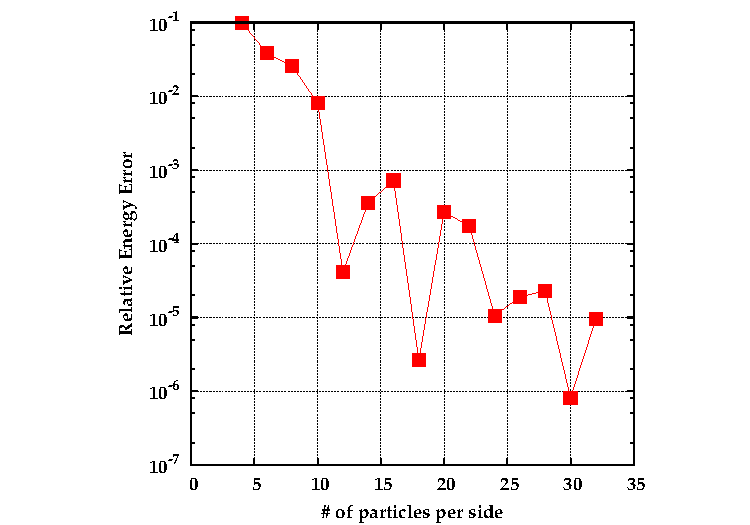
\includegraphics[width=10cm]{fig/p3m.pdf}
\caption{The relative error of the crystal energy as a function of the number of particles per side, where we assume that the number of the PM grids is $16^{3}$ and the cutoff radius is $3/16$.}
\label{fig:p3m}
\end{figure}
\clearpage

\ifCpp
%=========================
%   TreePM コードの解説
%=========================
\subsection{TreePM code} \label{subsec:TreePM}
In this section, we explain the usage of a FDPS extension ``Particle Mesh" (hereafter \textsf{PM}) using a sample program for TreePM(Tree-Particle-Mesh) method. This sample code performs cosmological $N$-body simulation using the TreePM method. In the TreePM method, the calculation of gravity is performed by splitting into the PP part and the PM part as in the $\mathrm{P^{3}M}$ method. Therefore, functions of FDPS used in the sample code is almost the same as the sample code for the $\mathrm{P^{3}M}$ method. The difference between the two is that the PP part is computed by the Tree method in the TreePM method while the $\mathrm{P^{3}M}$ method uses the direct summation for the PP part.

\subsubsection{Location of the sample code and the working directory}
The sample code is placed at \path{$(FDPS)/sample/c++/treepm}. Change the current directory to there.
As shown below, the sample code consists of several source files, of which the main body of the program is implemented in the files \texttt{treepm.hpp} and \texttt{treepm.cpp}.
\begin{screen}
\begin{verbatim}
$ cd (FDPS)/sample/c++/treepm
$ ls | awk '{print $0}'
IC/
Makefile
README_en.txt
README_ja.txt
constants.hpp
cosmology.hpp
fig/
make_directory.c
param_file_for_test.txt
prototype.h
result/
run_param.hpp
test.py*
timing.c
treepm.cpp
treepm.hpp
utils/
\end{verbatim}
\end{screen}

\subsubsection{Required header files}
In order to use the FDPS extension ``\textsf{PM}", we must include the header file \texttt{particle\_mesh.hpp} as well as \texttt{particle\_simulator.hpp}. These are described in the file \texttt{treepm.cpp}:
\begin{lstlisting}[caption=Include FDPS]
#include <particle_simulator.hpp>
#include <particle_mesh.hpp>
\end{lstlisting}

\subsubsection{User-defined classes}
In this section, we describe classes that you need to define in order to perform TreePM calculation using FDPS.

% FullParticle type
\subsubsubsection{FullParticle type}
You must define a \textsf{FullParticle} type. \textsf{FullParticle} type must have all physical quantities required to perform a calculation with the TreePM method. Listing \ref{treepm_FP} shows the implementation of \textsf{FullParticle} type in the sample code. In the code, it has member variables necessary for usual $N$-body simulations (\texttt{id}, \texttt{mass}, \texttt{eps}, \texttt{pos}, \texttt{vel}, \texttt{acc}). In addition, it has the following member variables: \texttt{acc\_pm} (stores the acceleration of the PM part), \texttt{H0} (stores the Hubble constant)、and \texttt{Lbnd} (stores the size of the simulation box in the unit of $\mathrm{Mpc\;h^{-1}}$). \textsf{FullParticle} type must have the following member functions to use the FDPS standard functions and the FDPS extension ``\textsf{PM}":
\begin{description}[leftmargin=*,itemsep=-1ex,style=nextline]
\item[\texttt{getCharge()}] required for FDPS to get the mass of particle
\item[\texttt{getChargeParticleMesh()}] required for the \textsf{PM} module to get the mass of particle
\item[\texttt{getPos()}] required for FDPS to get the position of particle
\item[\texttt{getRSearch()}] required for FDPS to get the cutoff radius
\item[\texttt{setPos()}] required for FDPS to write the position of particle recorded in \textsf{FullParticle} object
\item[\texttt{copyFromForce()}] required for FDPS to copy data from a \textsf{Force} object
\item[\texttt{copyFromForceParticleMesh()}] required for the \textsf{PM} module to write the result of Force calculation to \textsf{FullParticle} object
\end{description}
In addition, the sample uses file I/O functions of FDPS, which requires a user to define the following member functions:
\begin{itemize}[leftmargin=*,itemsep=-1ex]
\item \texttt{readBinary()}
\item \texttt{writeBinary()}
\end{itemize}
Note that the use of these file I/O functions is not necessary and user-defined I/O can be used.

\lstinputlisting[linerange={31-222},caption=\textsf{FullParticle} type,label=treepm_FP]{../../../../sample/c++/treepm/treepm.hpp}

% EssentialParticleI type
\subsubsubsection{EssentialParticleI type}
You must define a \textsf{EssentialParticleI} type and it must have all physical quantities as member variables that $i$ particle should have. Listing \ref{treepm_EPI} shows the implementation of \textsf{EssentialParticleI} type in the sample code. It must have member functions \texttt{copyFromFP()} (to copy data from a \textsf{FullParticle} object described above) and \texttt{getPos()} (to get the position of particle).

\lstinputlisting[linerange={231-247},caption=\textsf{EssentialParticleI} type,label=treepm_EPI]{../../../../sample/c++/treepm/treepm.hpp}

% EssentialParticleJ type
\subsubsubsection{EssentialParticleJ type}
You must define a \textsf{EssentialParticleJ} type and it must have all physical quantities as member variables that $j$ particle should have when the PP part of Force calculation is performed. Note that it is possible to define \textsf{EssentialParticleI} type so that it operates as \textsf{EssentialParticleJ} type as in the sample code for $\mathrm{P^{3}M}$ method (see \S~\ref{subsec:P3M}). Listing \ref{treepm_EPJ} shows the implementation of \textsf{EssentialParticleJ} type in this sample code. \textsf{EssentialParticleJ} type should have the following member functions:
\begin{description}[leftmargin=*,itemsep=-1ex,style=nextline]
\item[\texttt{getPos()}] required for FDPS to get the position of particle
\item[\texttt{getCharge()}] required for FDPS to get the mass of particle
\item[\texttt{copyFromFP()}] required for FDPS to copy data from \textsf{FullParticle} type to \textsf{EssentialParticleJ} type
\item[\texttt{getRSearch()}] required for FDPS to get the cutoff radius
\item[\texttt{setPos()}] required for FDPS to write the position of particle
\end{description}

\lstinputlisting[linerange={249-278},caption=\textsf{EssentialParticleJ} type,label=treepm_EPJ]{../../../../sample/c++/treepm/treepm.hpp}

% Force type
\subsubsubsection{Force type}
You must define a \textsf{Force} type and it must have all physical quantities that obtained as the results of the PP part of Force calculation. Listing \ref{treepm_force} shows the implementation of \textsf{Force} type. It must have a member function \texttt{clear()} in order to initialize or zero-clear the member variables that stored the results of accumulation operations.

\lstinputlisting[linerange={19-28},caption=\textsf{Force} type,label=treepm_force]{../../../../sample/c++/treepm/treepm.hpp}

% calcForceEpEp type
\subsubsubsection{calcForceEpEp type}
You must define a \textsf{calcForceEpEp} type and it must contain actual code for the PP part of Force calculation. Listing~\ref{treepm_calcForceEpEp} shows the implementation of \textsf{calcForceEpEp} type. In the sample code, \textsf{calcForceEpEp} type is implemented as a template function. Depending on the value of the macro \texttt{ENABLE\_PHANTOM\_GRAPE\_X86}, which determines whether to use the Phantom-GRAPE library, a different template function is used. In both cases, the arguments of the functions is an array of \textsf{EssentialParticleI} variables, the number of \textsf{EssentialParticleI} variables, an array of \textsf{EssentialParticleJ} variables, the number of \textsf{EssentialParticleJ} variables, an array of \textsf{Force} variables.

\lstinputlisting[linerange={344-365},caption=\textsf{calcForceEpEp} type,label=treepm_calcForceEpEp]{../../../../sample/c++/treepm/treepm.hpp}

The PP part of the TreePM method is a two-body interaction with cutoff as in the $\mathrm{P^{3}M}$ method. Hence, a cutoff function is involved in the calculation of gravitational acceleration. As explained in \S~\ref{subsubsubsec:p3m_calcForceEpEp}, the cutoff function must be the one that is constructed assuming that the particle shape function is $S2(r)$ (Hockney \& Eastwood 1988). The cutoff function is implemented as the function \texttt{gfactor\_S2()} for the case where the Phantom-GRAPE library is not used. In using the Phantom-GRAPE library, you do not have to implement the cutoff function because the library computes the interaction taking into account cutoff. In this case, you must call the library's API \texttt{pg5\_gen\_s2\_force\_table()} before the Force calculation in order to give the value of the cutoff radius to the library. In the sample code, the call of the API is performed at the main function:
\begin{lstlisting}
#ifdef ENABLE_PHANTOM_GRAPE_X86 
    //g5_open();
    pg5_gen_s2_force_table(EPS_FOR_PP, 3.0/SIZE_OF_MESH);
#endif
\end{lstlisting}

% Main body of the program
\subsubsection{Main body of the program}
In this section, we explain in detail the main body of the program. Before going into details, we first give a simple explanation about the content and the structure of the sample code. As described in the beginning of \S~\ref{subsec:TreePM}, this code performs a cosmological $N$-body simulation using the TreePM method. The code supports three different types of initial condition files:
\begin{enumerate}[leftmargin=*,itemsep=-1ex,label=(\alph*)]
\item Initial condition files used in the Santa Barbara Cluster
  Comparison Test
  (\href{http://iopscience.iop.org/article/10.1086/307908/meta}{Frenk
    et al.[1999, ApJ, 525, 554]}). These initial condition files are
  available at \url{https://v2.jmlab.jp/owncloud/index.php/s/XnzvW5XAYwfqZYQ?path=%2Fsb}, where \path{ic_sb128.tar} for $N=128^3$ and \path{ic_sb256.tar} for $N=256^3$.
\item Initial condition files described in the same format as the above test
\item Random distribution of particles
\end{enumerate}
You must pass the absolute PATH of an initial condition file as the runtime command-line argument. Then, the program reads the given initial condition file and automatically identifies the type of initial condition ((a)-(c)). After setting the initial condition, the code numerically integrates the motions of particles to the finish time (specified by the redshift $z$) described in the file using the TreePM method. For the details of the format of initial condition file, please see \path{$(FDPS)/sample/c++/treepm/README_en.txt}. Note that an example of the initial condition file for the case (a) is given at \path{$(FDPS)/sample/c++/treepm/result/input.para}.

The structure of the sample code is as follows::
\begin{enumerate}[leftmargin=*,itemsep=-1ex,label=(\arabic*)]
\item Create and initialize FDPS objects
\item Initialize the Phantom-GRAPE library (if needed)
\item Read the initial condition file 
\item Integrate the motions of particles in time to the finish time
\end{enumerate}

In the followings, we explain in detail each step described above.

\subsubsubsection{Initialization and Termination of FDPS}
First, you must initialize FDPS by the following code.
\begin{lstlisting}[caption=Initialization of FDPS]
PS::Initialize(argc, argv);
\end{lstlisting}

Once started, FDPS should be terminated explicitly. In this sample, FDPS is terminated just before the termination of the program. Hence, you need to write the following code at the end of the main function.
\begin{lstlisting}[caption=Termination of FDPS]
PS::Finalize();
\end{lstlisting}

\subsubsubsection{Creation and Initialization of FDPS objects}
After the initialization of FDPS, a user need to create the objects used to talk to FDPS. In this section, we describe how to create and initialize these objects.

\subsubsubsubsection{Creation of necessary FDPS objects}
In the calculation using the TreePM method, we must create objects of the \textsf{FullParticle} class, the \textsf{DomainInfo} class, the \textsf{TreeForForceLong} class (used in the PP part), and the \textsf{ParticleMesh} class (used in the PM part). In the sample code, these objects are created in the main function described in \texttt{treepm.cpp}:
\begin{lstlisting}[caption=Creation of FDPS objects]
int main(int argc, char **argv)
{
   PS::PM::ParticleMesh pm;
   PS::ParticleSystem<FPtreepm> ptcl;
   PS::DomainInfo domain_info;
   PS::TreeForForceLong<Result_treepm, EPItreepm, EPJtreepm>::MonopoleWithCutoff treepm_tree;

}
\end{lstlisting}
Note that the above code is the one that is constructed by collecting the parts of object creation.

\subsubsubsubsection{Initialization of FDPS objects}
Almost all of FDPS objects must be initialized before they are used in a user code. Of four objects described in previous section, the \textsf{ParticleMesh} object is the only object that does not require an explicit initialization. The initialization of the other objects is done by the \texttt{initialize} method. In the following, we show an excerpt of the sample code where the initializations are performed:
\begin{lstlisting}[caption=Initialization of FDPS objects]
int main(int argc, char **argv)
{
   // Initialize ParticleSystem
   ptcl.initialize();

   // Initialize DomainInfo
   domain_info.initialize();  
   domain_info.setBoundaryCondition(PS::BOUNDARY_CONDITION_PERIODIC_XYZ);
   domain_info.setPosRootDomain(PS::F64vec(0.0, 0.0, 0.0), 
                                PS::F64vec(1.0, 1.0, 1.0));
                                
   // Initialize Tree
   treepm_tree.initialize(3*ptcl.getNumberOfParticleGlobal(),
                          this_run.theta);
}
\end{lstlisting}

\begin{itemize}[leftmargin=*,itemsep=-1ex]
% ParticleSystem
\item The initialization of a \textsf{ParticleSystem} object is simply done by calling \texttt{initialize} method without any arguments.
% DomainInfo
\item As for a \textsf{DomainInfo} object, we must set the boundary condition and the size of the simulation box after calling \texttt{initialize} method. These are done by calling \texttt{setBoundaryCondition} and \texttt{setPosRootDomain} methods.
% TreeForForceLong
\item We must pass a rough number of particles to the \texttt{initialize} method of a \textsf{TreeForForceLong} object as the first argument. In this sample code, we pass a value three times larger than the total number of the particles. We can specify the value of the opening angle criterion $\theta$ used in the force calculation of the tree method via the second argument. Note that the object \texttt{this\_run} is used to store a set of parameters such as $\theta$ that control the simulation.
\end{itemize}


\subsubsubsection{Initial Condition}
An parameter file that specifies an initial condition is read in the function \texttt{read\_param\_file()} described in the main function:
\begin{lstlisting}
read_param_file(ptcl, this_run, argv[1]);
\end{lstlisting}
This function reads the parameter file specified by the command line arguments and sets the particle information such as mass and position to the \textsf{ParticleSystem} object based on the parameter file. After that, the sample code performs domain decomposition and particle exchange using FDPS APIs. In the following, we explain these APIs in detail. 

\subsubsubsubsection{Domain Decomposition}
The sample code first perform domain decomposition, which is done by calling the \texttt{decomposeDomainAll} method (see the \texttt{main} function):
\begin{lstlisting}[caption=Domain Decomposition]
domain_info.decomposeDomainAll(ptcl);
\end{lstlisting}
This method divides the entire of the domain based on a given particle distribution. Hence, we need to pass a \textsf{ParticleSystem} object to this method. 

\subsubsubsubsection{Particle Exchange}
Then, the code performs particle exchange, which is done by calling the \texttt{exchangeParticle} method (see the \texttt{main} function):
\begin{lstlisting}[caption=Particle Exchange]
ptcl.exchangeParticle(domain_info);
\end{lstlisting}
where we pass a \textsf{DomainInfo} object to this method because the method needs to know the information of domain decomposition in advance.

\subsubsubsection{Interaction Calculation}
After that, the code performs interaction calculation to determine the accelerations at the initial time.
In the following, we show our implementation of interaction calculation.
In this code, the \texttt{calcForceAllAndWriteBack} method of the \textsf{TreeForForceLong} object is used to calculate the PP part of the force calculation. This method automatically stores the results into the member variable \texttt{acc} of the \textsf{ParticleSystem} object. As for the PM part of the force calculation, we use the \texttt{calcForceAllAndWriteBack} method of the \textsf{ParticleMesh} object. Likewise, this method automatically stores the results of the PM part into the member variable \texttt{acc\_pm} of the \textsf{ParticleSystem} object.

\begin{lstlisting}[caption=Interaction Calculation]
//* PP part
treepm_tree.calcForceAllAndWriteBack
    (calc_pp_force<EPJtreepm>(),
     calc_pp_force<PS::SPJMonopoleCutoff>(),
     ptcl,
     domain_info);
 
//* PM part
pm.calcForceAllAndWriteBack(ptcl, domain_info); 
\end{lstlisting}

\subsubsubsection{Time Integration}
The sample code uses the Leapfrog time integrator to perform time integration (the details of the method is described in \S~\ref{s4sec:nbody_time_integration}). The $D(\cdot)$ operator, which integrates the positions of particles in time, is implemented as the function \texttt{drift\_ptcl}, while the $K(\cdot)$ operator, which integrates the velocities of particles in time, is implemented as the function \texttt{kick\_ptcl}. The effects of cosmic expansion is taken into account in the function \texttt{kick\_ptcl}. The time evolution of the scale factor and the Hubble parameter is done by the \texttt{update\_expansion} method of the \texttt{this\_run} object.

\subsubsection{Compile}
As explained in README.txt, you must edit \texttt{Makefile} in \texttt{src} directory appropriately to adapt to your computer environment. Then, run \texttt{make} command to compile the sample code. Note that this code uses FFTW library and therefore you have to install it in advance. The execution file \texttt{treepm} will be created if the compilation is succeeded.

\subsubsection{Execution}
We must run the program using MPI with the number of MPI processes is equal to or greater than 2, because of the specification of FDPS extension "ParticleMesh" module. Therefore, you should run the following command:
\begin{screen}
\begin{verbatim}
$ MPIRUN -np NPROC ./treepm
\end{verbatim}
\end{screen}
where "MPIRUN" represents the command to run a program using MPI such as \texttt{mpirun} or \texttt{mpiexec}, and "NPROC" is the number of MPI processes.

\subsubsection{Confirmation of the result}
After the simulation is completed, the results will be output at the directory specified in the parameter file.
Figure~\ref{fig:treepm} shows the time evolution of column density distribution of dark matter in a Santa Barbara Cluster Comparison test with $256^{3}$ particles.

\begin{figure}[h]
\centering
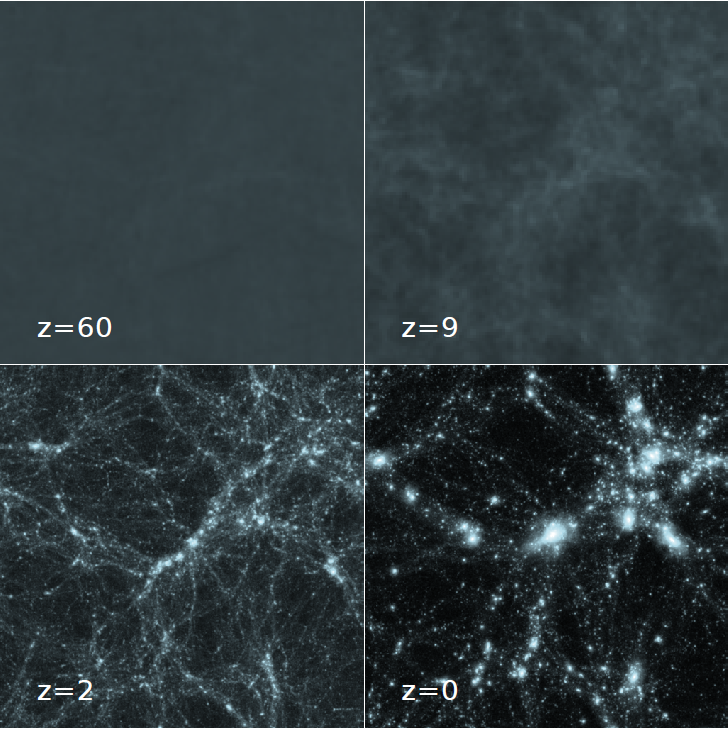
\includegraphics[width=0.666\linewidth]{./fig/sb256.png}
\caption{Time evolution of particle density of Santa Barbara Cluster Comparison test (the number of particles is $256^{3}$)}
\label{fig:treepm}
\end{figure}

\endifCpp % End of \ifCpp enclosing the subsection of TreePM code